%
% This is the LaTeX template file for lecture notes for CS294-8,
% Computational Biology for Computer Scientists.  When preparing 
% LaTeX notes for this class, please use this template.
%
% To familiarize yourself with this template, the body contains
% some examples of its use.  Look them over.  Then you can
% run LaTeX on this file.  After you have LaTeXed this file then
% you can look over the result either by printing it out with
% dvips or using xdvi.
%
% This template is based on the template for Prof. Sinclair's CS 270.

\documentclass[twoside, 12pt]{article}
\usepackage{graphics}
\setlength{\oddsidemargin}{0.25 in}
\setlength{\evensidemargin}{-0.25 in}
\setlength{\topmargin}{-0.6 in}
\setlength{\textwidth}{6.5 in}
\setlength{\textheight}{8.5 in}
\setlength{\headsep}{0.75 in}
\setlength{\parindent}{0 in}
\setlength{\parskip}{0.1 in}


%
% The following commands set up the lecnum (lecture number)
% counter and make various numbering schemes work relative
% to the lecture number.
%
\newcounter{lecnum}
\renewcommand{\thepage}{\thelecnum-\arabic{page}}
\renewcommand{\thesection}{\thelecnum.\arabic{section}}
\renewcommand{\theequation}{\thelecnum.\arabic{equation}}
\renewcommand{\thefigure}{\thelecnum.\arabic{figure}}
\renewcommand{\thetable}{\thelecnum.\arabic{table}}

%
% The following macro is used to generate the header.
%
\newcommand{\lecture}[4]{
   \pagestyle{myheadings}
   \thispagestyle{plain}
   \newpage
   \setcounter{lecnum}{#1}
   \setcounter{page}{1}
   \noindent
   \begin{center}
   \framebox{
      \vbox{\vspace{2mm}
    \hbox to 6.28in { {\bf UGBA 141 Production and Operations Management
                        \hfill Spring 2022} }
       \vspace{4mm}
       \hbox to 6.28in { {\Large \hfill Cheatsheet #1: #2  \hfill} }
       \vspace{2mm}
       \hbox to 6.28in { {\it 
       Lecturer: #3 
       \hfill 
       GSI: #4} }
      \vspace{2mm}}
   }
   \end{center}
%  \markboth{Lecture #1: #2}{Lecture #1: #2}
%   {\bf Disclaimer}: {\it These notes have not been subjected to the
%   usual scrutiny reserved for formal publications.  They may be distributed
%   outside this class only with the permission of the Instructor.}
   \vspace*{4mm}
}

%
% Convention for citations is authors' initials followed by the year.
% For example, to cite a paper by Leighton and Maggs you would type
% \cite{LM89}, and to cite a paper by Strassen you would type \cite{S69}.
% (To avoid bibliography problems, for now we redefine the \cite command.)
% Also commands that create a suitable format for the reference list.
\renewcommand{\cite}[1]{[#1]}
\def\beginrefs{\begin{list}%
        {[\arabic{equation}]}{\usecounter{equation}
         \setlength{\leftmargin}{2.0truecm}\setlength{\labelsep}{0.4truecm}%
         \setlength{\labelwidth}{1.6truecm}}}
\def\endrefs{\end{list}}
\def\bibentry#1{\item[\hbox{[#1]}]}

%Use this command for a figure; it puts a figure in wherever you want it.
%usage: \fig{NUMBER}{SPACE-IN-INCHES}{CAPTION}
\newcommand{\fig}[3]{
			\vspace{#2}
			\begin{center}
			Figure \thelecnum.#1:~#3
			\end{center}
	}
% Use these for theorems, lemmas, proofs, etc.
\newtheorem{theorem}{Theorem}[lecnum]
\newtheorem{lemma}[theorem]{Lemma}
\newtheorem{proposition}[theorem]{Proposition}
\newtheorem{claim}[theorem]{Claim}
\newtheorem{corollary}[theorem]{Corollary}
\newtheorem{definition}[theorem]{Definition}
\newenvironment{proof}{{\bf Proof:}}{\hfill\rule{2mm}{2mm}}


% self added package
\usepackage{amsmath}
 \usepackage{graphicx}

% **** IF YOU WANT TO DEFINE ADDITIONAL MACROS FOR YOURSELF, PUT THEM HERE:

\begin{document}
%FILL IN THE RIGHT INFO.
%\lecture{**LECTURE-NUMBER**}{**DATE**}{**LECTURER**}{**SCRIBE**}
\lecture{2}{Quality}{Park Sinchaisri}{Hansheng Jiang}
%\footnotetext{These notes are partially based on those of Nigel Mansell.}

% **** YOUR NOTES GO HERE:

% Some general latex examples and examples making use of the
% macros follow.  
%**** IN GENERAL, BE BRIEF. LONG SCRIBE NOTES, NO MATTER HOW WELL WRITTEN,
%**** ARE NEVER READ BY ANYBODY.

\begin{enumerate}


\item {\bf Control charts}

In building control charts, we usually have access to data from multiple periods. The sample from one period may contains multiple data points, and the number of data points in one sample is called sample size. For each sample, we can compute its mean $\overline{X}$, range $R$,  propostion of defects $p$, and count of defects $c$. Taking the average of $\bar{X}$,  $R$,  $p$, and  $c$ across multiple periods, we get  $\overline{\overline{X}}$,  $\overline{R}$,  $\overline{p}$, and  $\overline{c}$.

The sample size affects the UCL and LCL computation of mean charts, $R$-charts, and $p$-charts. The dependence of $p$-charts on the sample size is clear from the table below. For mean charts and $R$-charts, the control chart constants $A_2, D_3,D_4$ are decided by the sample size (See the \texttt{Table of Control Chart Constants} in bcourses/Files/05 Quality I/). 

\begin{figure}[!ht]
	\centering
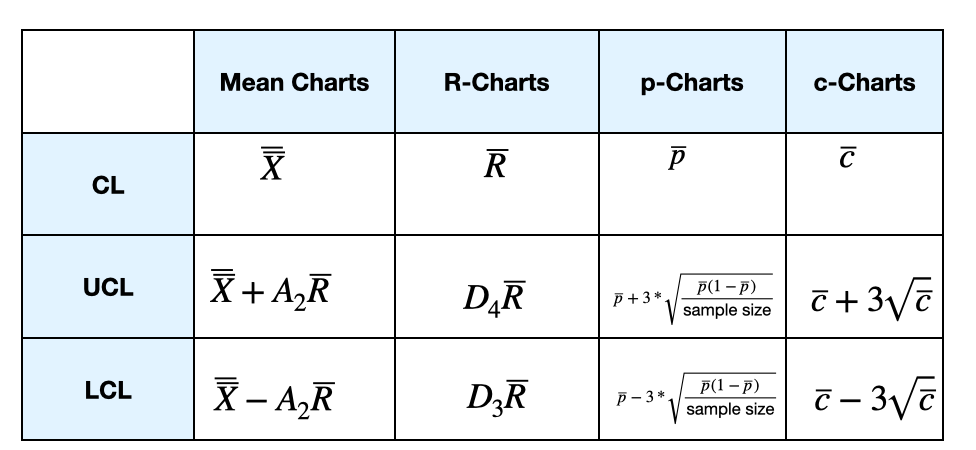
\includegraphics[width = 0.9\textwidth]{control_chart_screenshot}
\end{figure}



\item {\bf Capability analysis}
\begin{enumerate}
	\item For centered process ($\overline{X} = \frac{\text{USL}+\text{LSL}}{2}$), the process capability measure is $C_p$, calculated as
	\[
	C_p = \frac{\text{USL}-\text{LSL}}{6 \hat{\sigma}}.
	\]
	\item For off-centered process ($\overline{X} \neq \frac{\text{USL}+\text{LSL}}{2}$), the process capability measure is $C_{pk}$, calculated as
	\[
	C_{pk} = \min \left\{ \frac{\text{USL} - \overline{X}}{3 \hat{\sigma}},  \frac{\overline{X}-\text{LSL}}{3 \hat{\sigma} } \right\}
	\]
	\item $\hat{\sigma}$ is  estimated standard deviation. If $\hat{\sigma}$ is not given, we pool all data points together to compute the standard deviation using formula
	\[
	\hat{\sigma} = \sqrt{ \frac{\sum_{i=1}^N (X_i - \overline{X})^2}{N-1}},
	\]
	where there is a slight abuse of notation as the mean is named $\overline{\overline{X}}$ in the mean-charts.
\end{enumerate}

\end{enumerate}















\section*{References}
\beginrefs


\bibentry{TC2006}{\sc C.~Terwiesch} and {\sc G.~Cachon}, 
  Matching supply with demand: An introduction to operations management (Chapter 7), {McGraw-Hill~2006}
  
\bibentry{SG2018}{\sc R.~Schroeder} and {\sc S. M. ~Goldstein}, 
Operations Management in the Supply Chain (Chapter 8 and 9), {McGraw-Hill~2018}

\endrefs


\end{document}





